% ============================================================
%  Physical Review B style article
%  Compile with pdflatex (run TWICE for references)
% ============================================================
\documentclass[
    aps,
    prb,
    reprint,           % single-column, double-spaced, for submission
    % twocolumn,       % uncomment for the published two-column look
    superscriptaddress,% affiliations as superscript numbers
    amsmath,amssymb,
    floatfix
]{revtex4-1}

% ---------- Packages ----------
\usepackage{graphicx}      % figures
\usepackage{dcolumn}       % decimal-aligned table columns
\usepackage{bm}            % bold math
\usepackage{amsmath}
\usepackage{amssymb}
\usepackage{hyperref}      % clickable links in PDF (optional)
\usepackage{color}
\usepackage{siunitx}       % SI units (\SI{1}{\kelvin})
\usepackage{physics}       % \dv, \pdv, \bra, \ket, ...
\usepackage{url}
\usepackage{subcaption}   % modern, works with revtex4-2
\usepackage{graphicx}     % already present
\usepackage{adjustbox}

% ---------- Custom commands (optional) ----------
\newcommand{\md}{\mathrm{d}}
\newcommand{\ee}{\mathrm{e}}
\newcommand{\ii}{\mathrm{i}}
\newcommand{\kB}{k_{\mathrm{B}}}
\newcommand{\Jij}{J_{ij}}
\newcommand{\sgn}{\operatorname{sgn}}

% ============================================================
\begin{document}

% ---------- Title ----------
\title{Analysis of phase transition in a nanomagnetic artificial Hopfield network}

% ---------- Authors ----------
\author{Kim Chol-jun}
\email{kim.cc@dvfu.ru}
\affiliation{Institute of High Technologies and Advanced Materials, Far Eastern Federal University, Russian Federation}
\affiliation{Physic Faculty, {\bf Kim Il Sung} University, Pyongyang, DRP of Korea}

\author{Konstantin Valentinovich Nefedev}
\affiliation{Institute of High Technologies and Advanced Materials, Far Eastern Federal University, Russian Federation}


% ---------- Dates ----------
\date{\today}

% ---------- Abstract ----------
\begin{abstract}
...
\end{abstract}

% ---------- PACS (optional, PRB still allows) ----------
% \pacs{75.10.Nr, 75.50.Lk, 75.40.Mg}

% ---------- Make title ----------
\maketitle

% ============================================================
\section{Introduction}
\label{sec:intro}


% ============================================================
\section{Model and Formalism}
\label{sec:model}

Suppose that every particle has a single Ising spin ($\sigma _i=\pm 1$), the norm of its magnetic momentum is $\mu$ and they interact with each other through dipolar interaction. The Hamiltonian of the dipolar Ising system can be defined 
\begin{equation}
\mathcal{H}=\sum_{i<j} J_{ij}\text{\,}{\sigma }_i{\sigma }_j\text{\; \,}-\text{\; \,}\mu \sum_i {\sigma }_i\text{\,}({\widehat{n}}_i\cdot \mathbf{h}), 	
 \label{eq:ham1}
\end{equation}
where $\mathbf{h}$ is an external magnetic field and $J_{ij}$is the dipole–dipole interaction:
\begin{equation}
J_{ij}=\frac{{\mu }_{0}{\mu }^{2}}{4\pi }\text{\,}\frac{{\widehat{n}}_i\cdot {\widehat{n}}_j\text{\; \,}-\text{\; \,}3({\widehat{n}}_i\cdot {\widehat{r}}_{ij})({\widehat{n}}_j\cdot {\widehat{r}}_{ij})}{r_{ij}^{\text{\; \,}3}},	
 \label{eq:dipterm}
\end{equation}
where ${\widehat{r}}_{ij}$ is the unit vector of displacement between $i$ and $j$-th particles and ${\widehat{n}}_i$ is the unit vector of the spin which seems along the easy axis of the particle. No exchange is included – only dipolar.

Without loss of generality, we can assume that the external field is directed in the $y$-axis: $\mathbf{h}=h_{y}\widehat{y}$. Then the corresponding magnetization is as follows: 
\begin{equation}
M_{y}=\mu \sum_i {\sigma }_i({\widehat{n}}_i)_{y} 
 \label{eq:mag-y}
\end{equation}
Defining a new variable
\begin{equation}
{\tau }_i\equiv \sigma_i({\widehat{n}}_i)_{y}, 	
 \label{eq:tau}
\end{equation}
the magnetization can be rewritten as
\begin{equation}
M_{y}=\mu \sum_i {\tau }_i. 
 \label{eq:mag-gaugeinv-y}
\end{equation} 
The magnetic susceptibility is defined from the physical magnetization as a linear response:
\begin{equation}
{\chi }_{yy}=\frac{\partial M_{y}}{\partial h_{y}}\Big|_{h_{y}=0}.		
 \label{eq:susc1}
\end{equation}
If we consider a thermal dependency of the susceptibility, we can get the following definition of the isothermal susceptibility: how the average magnetization changes when you apply a tiny external field:
\begin{equation}
{\chi }_{yy}(T)=\frac{\partial \langle M_y\rangle}{\partial h_y} \Big|_{h_y=0}.		
 \label{eq:susc-ther}
\end{equation}
According to the fluctuation–dissipation theorem (FDT), we can obtain
\begin{equation}
{\chi }_{yy}\left(T\right)=\beta {\left(\langle M_y^{2}\rangle-\langle M_y\rangle^{2}\right)}_{h=0},
 \label{eq:mag-fdt}
\end{equation}
where $\beta =1/(k_{B}T)$. $\langle \cdot \rangle$ stands for the thermal average: for an observable A, it is defined as
\begin{equation}
\langle \mathrm{A}\rangle =\frac{1}{Z}\text{\,}\mathrm{Tr}[\mathrm{A}\ e^{-\beta \mathcal{H}}], 
\label{eq:mag-fdt}
\end{equation}
where 
\begin{equation}
Z=\mathrm{Tr}\text{\,}e^{-\beta \mathcal{H}}	
\end{equation}
is the canonical partition function and Tr means the trace, that is, the sum over all configurations (for example, over $2^N$ configurations for $N$ spins):
\begin{equation}
\mathrm{Tr}\left[\cdots \text{\,}\right]\text{\; \,}\equiv \text{\; \,}\sum_{\left\{\sigma \right\}} (\left.\cdots \text{\,}\right)=\sum_{{\sigma }_1=\pm 1} \cdots \sum_{{\sigma }_{N}=\pm 1} (\left.\cdots \text{\,}\right)		
 \label{eq:Trdef}
\end{equation}
A similar formula can be obtained for the heat capacity as well:
\begin{equation}
C=\frac{\langle {\mathcal{H}}^{2}\rangle -{\langle \mathcal{H}\rangle }^{2}}{k_{B}T^{2}}  
\qq{\text{or}}  
C=\frac{\langle E^{2}\rangle -{\langle E\rangle }^{2}}{k_{B}T^{2}}\ 
 \label{eq:cap-fdt},
\end{equation}
wher $E$ is the energy of spin state.

The magnetic susceptibility and the heat capacity mentioned above are extensive observables, depending on the volume or the number of particles. In this paper, we consider only the observables per spin or particle:
\begin{equation}
 \chi_{\tau }\left(T\right)=\frac{\langle M_y^{2}\rangle-\langle M_y\rangle^{2}}{k_{B}TN},
  \label{eq:mag-per-spin}
\end{equation}
\begin{equation}
C=\frac{\langle E^{2}\rangle -{\langle E\rangle }^{2}}{k_{B}T^{2}N},
 \label{eq:cap-per-spin}
\end{equation}
where $N$ is the number of particles. 

The Edwards-Anderson (EA)  order parameter is an important quantitative measure for confirming the existence of the spin-glass phase. In their original paper~\cite{EA1975}, they defined the order parameter as the long-time / thermal average of a single spin's autocorrelation:
\begin{equation}
q_{EA}=\underset{t\rightarrow \infty }{\lim}\overline{\langle s_i(0) s_i\left(t\right)\rangle }	
 \label{eq:15}
\end{equation}
where $\langle \cdot\rangle$is the thermal average at fixed disorder (one sample), $\overline{(\cdot )}$is the disorder average (average over random bond realizations). This quantity is difficult to calculate in the real simulation. Under the assumption of the translational invariance of the average, we could replace this with the thermal average, the disorder average (over the sub-lattices) and/or the site average (per spin) as follows:
\begin{equation}
q=\underset{\text{disorder}}{\underbrace{\frac{1}{M}\sum_{a=1}^{M}}}\underset{\text{thermal}}{\underbrace{\sum_{s_1,s_2} p_{s_1}^{(a)}p_{s_2}^{(a)}}}\underset{\text{site}}{\underbrace{\frac{1}{N}\sum_{i=1}^{N}}}s_i^{\left(s_1\right)}s_i^{\left(s_2\right)},
 \label{eq:16}
\end{equation} 
where $a$ represents a sub-lattice (with a given size), $p_{s_j}^{(a)}$ is Boltzmann weight of configuration $s_1$ and $i$ is the site number. But if we consider two states: an original (random) state and a new state that includes an odd number of spins flipped from the original one, they give opposite overlap and are canceled out by each other in the sum. Thus, enumeration over all possible states gives $q_{\mathrm{EA}}=0$. Therefore, we introduce $q^2$ or $|q|$:
\begin{equation}
 q^{2}=\underset{\text{disorder}}{\underbrace{\frac{1}{M}\sum_{a=1}^{M}}}\underset{\text{thermal}}{\underbrace{\sum_{s_1,s_2} p_{s_1}^{(a)}p_{s_2}^{(a)}}}\underset{\text{site}}{\underbrace{\frac{1}{N}\sum_{i=1}^{N}}}{\left(s_i^{\left(s_1\right)}s_i^{\left(s_2\right)}\right)}^{2},
  \label{eq:17}
\end{equation}
 \begin{equation}
\left|q\right|=\underset{\text{disorder}}{\underbrace{\frac{1}{M}\sum_{a=1}^M}}\underset{\text{thermal}}{\underbrace{\sum_{s_1,s_2} p_{s_1}^{(a)}p_{s_2}^{(a)}}}\underset{\text{site}}{\underbrace{\frac{1}{N}\sum_{i=1}^{N}}}\left|s_i^{\left(s_1\right)}s_i^{\left(s_2\right)}\right|.
 \label{eq:18}
\end{equation}
In Monte-Carlo (MC) simulation, $\sum_{s_1,s_2} p_{s_1}^{(a)}p_{s_2}^{(a)}$ can be replaced by the sum for all pairs of the accepted states.

$m$ or a magnetization order parameter is defined as:
\begin{equation}
M=\frac{1}{N}\sum_{i=1}^{N} \langle s_i\rangle,	
 \label{eq:19}
\end{equation}
where $N$ is number of spins and $\langle\cdot\rangle$ denotes the thermal average.

The spin–spin correlation function in a spin glass is determined by
\begin{equation}
G(r)={\overline{\langle s_is_j\rangle }}_{\mid r_i-r_j\mid =r}	
  \label{eq:20}
\end{equation}
where $\langle\cdot\rangle$ stands for the thermal average and $\overline{(\cdot )}$ for the average over pairs $(i, j)$ at distance $r$, dividing by the total number of pairs $(i, j)$. So, it can be calculated by
\begin{equation}
G(r)=\frac{1}{N_p(r)}\sum_{i,j:\mid r_i-r_j\mid \approx r}\frac{1}{Z}\sum_{\{s\}} s_i s_j e^{-\beta E\left({s}\right)} 
  \label{eq:21}
\end{equation}
or 
\begin{equation}
G(r)\text{\; \,}=\text{\; \,}\frac{1}{N_p(b)}\sum_{\left(i,\; j\right)\in b}\underset{\text{thermal\ average}}{\underbrace{\frac{1}{M}\sum_{a=1}^{M} s_i^{(a)}s_j^{(a)}}},
  \label{eq:22}
\end{equation}
where $N_p(r)$ or $N_p(b)$ is the number of pairs with distance in the bin at $r$ or $b$-th bin and $Z=\sum_{\{s\}} e^{-\beta E\left({s}\right)}$ is the partition function.
In addition to this, we could consider a $q-q$ correlation function as well:
\begin{equation}
G_{SG}(r)={\overline{\langle q_iq_j\rangle }}_{\mid r_i-r_j\mid =r}, 
  \label{eq:23}
\end{equation}
which can be calculated numerically as
\begin{equation}
G_{SG}(r)=\frac{1}{N_p(r)}\sum_{\left(i,\; j\right)\in r}\sum_{a} \sum_{b} p_{a}p_{b}q_i^{(a,b)}q_j^{(a,b)}
  \label{eq:24}
\end{equation}
or
\begin{equation}
G_{SG}\left(r_{b}\right)=\frac{1}{N_p(b)}\sum_{\left(i,\; j\right)\in b} \frac{1}{N_{\left(a,\; b\right)}}\sum_{\left(a,\; b\right)} q_i^{(a,b)}q_j^{(a,b)},
  \label{eq:25}
\end{equation}
where $q_i^{(a,b)}=s_i^{(a)}s_i^{(b)}$.

The correlation length $\xi$ is defined through the decay of the two-point correlation function:
\begin{equation}
G(r)\sim e^{-r/\xi }\ \text{as\ }r\rightarrow \infty 
  \label{eq:26}
\end{equation}
So $\xi$ is the characteristic distance over which two spins remain correlated.
Given $G(r)$, there are two standard ways to extract $\xi$. One way is by the second-moment estimator:
\begin{equation}
{\xi }^{2}=\frac{\sum_{r} r^{2}\text{\,}G(r)}{\sum_{r} G(r)},
  \label{eq:27}
\end{equation}
which does not require fitting, so it might be standard in modern spin-glass simulations. Another way is through the exponential fit: fitting $\log{G}(r)$vs $r$ to a line
\begin{equation}
\log{G}(r)=\log{A}-r/\xi,
  \label{eq:28}
\end{equation}
we can know $-1/\xi$ by the slope.
From both $G(r)$ and $G_{SG}(r)$, we could obtain $\xi$ and $\xi_{SG}$, respectively. 

% ============================================================


\section{Analysis of the experiment in \cite{Saccone2022}}
\label{sec:anal}
As a physical experiment, we analyze Saccone et al's experiment~\cite{Saccone2022}. They fabricated nanomagnetic Hopfield networks consisting of permalloy (Ni$_{80}$Fe$_{20}$) Ising-type nanomagnets with lengths $L$ = 300 nm, widths $W$ = 100 nm, and thicknesses $t$ = 2.7 nm. Every particle has the magnetic moment $\mu_{ref} = 5.41 \times 10^{-18}$ Am$^2$.

\begin{figure*}[t]
    \centering

    % ---- Subfigure (a) ----
    \begin{subfigure}[b]{0.4\textwidth}
    	%\adjincludegraphics[width=\linewidth]{fig/Thick008.png}
    	% \adjincludegraphics[width=0.7\textwidth]{fig/Thick008.png}
        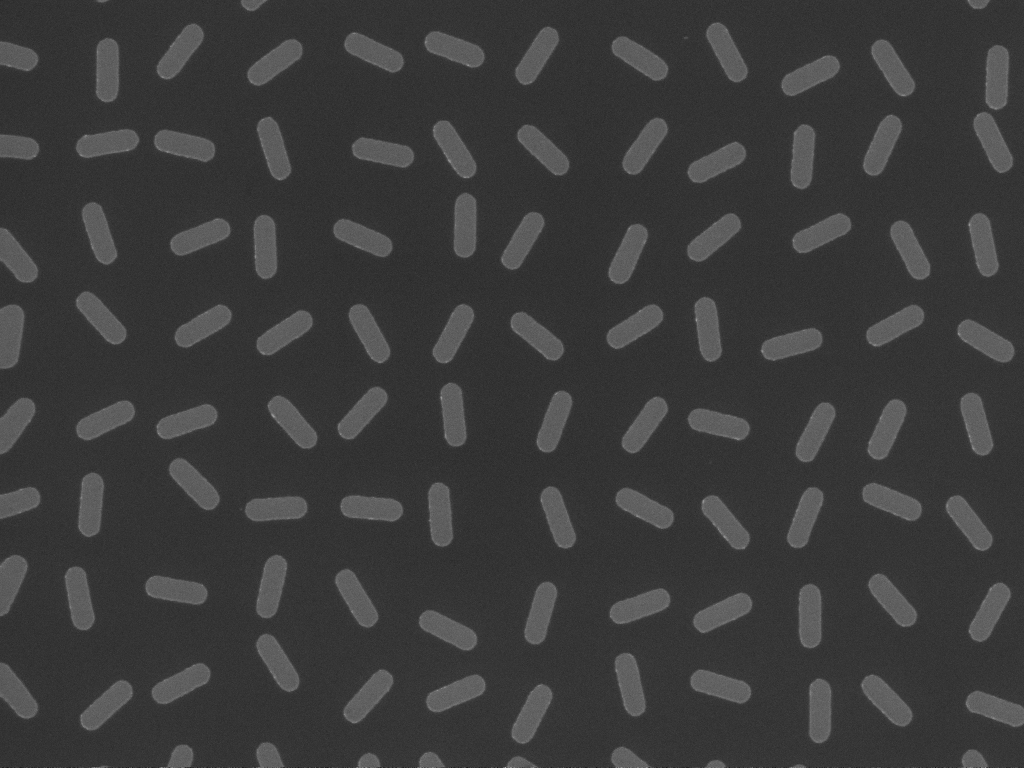
\includegraphics[width=\linewidth]{fig/Thick008.png}
        \caption{}
        \label{fig:sac1a}
    \end{subfigure}
    \quad
    % \hfill
    % ---- Subfigure (b) ----
    \begin{subfigure}[b]{0.4\textwidth}
    	% 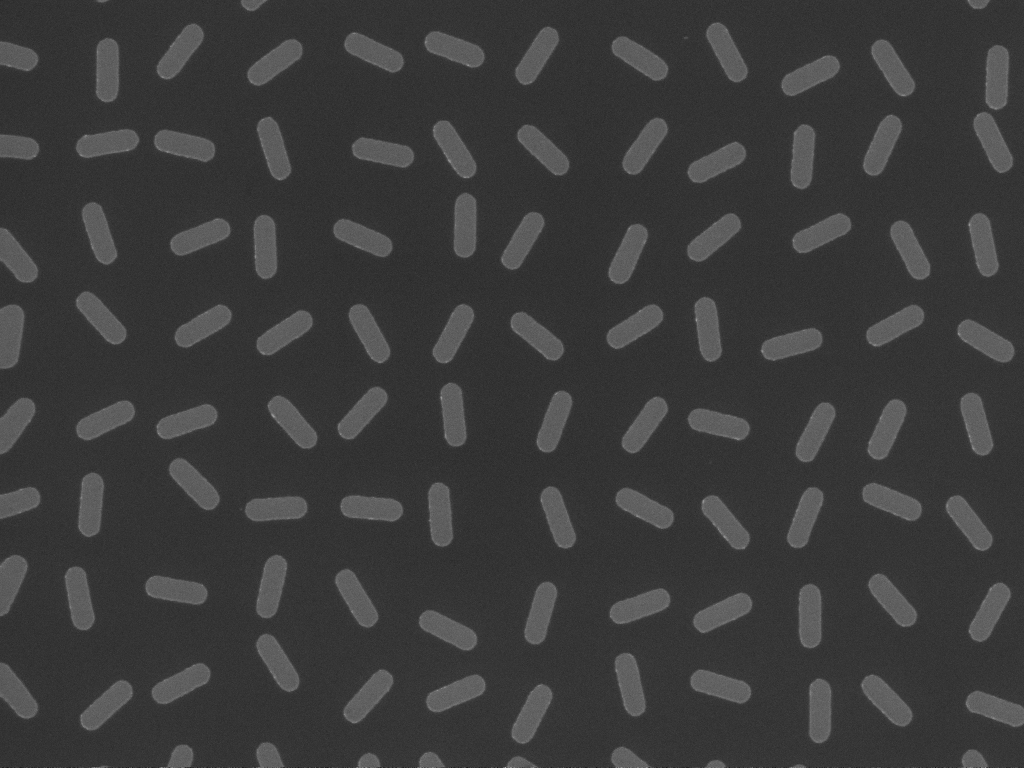
\includegraphics[width=\linewidth]{fig/Thick008.png}
        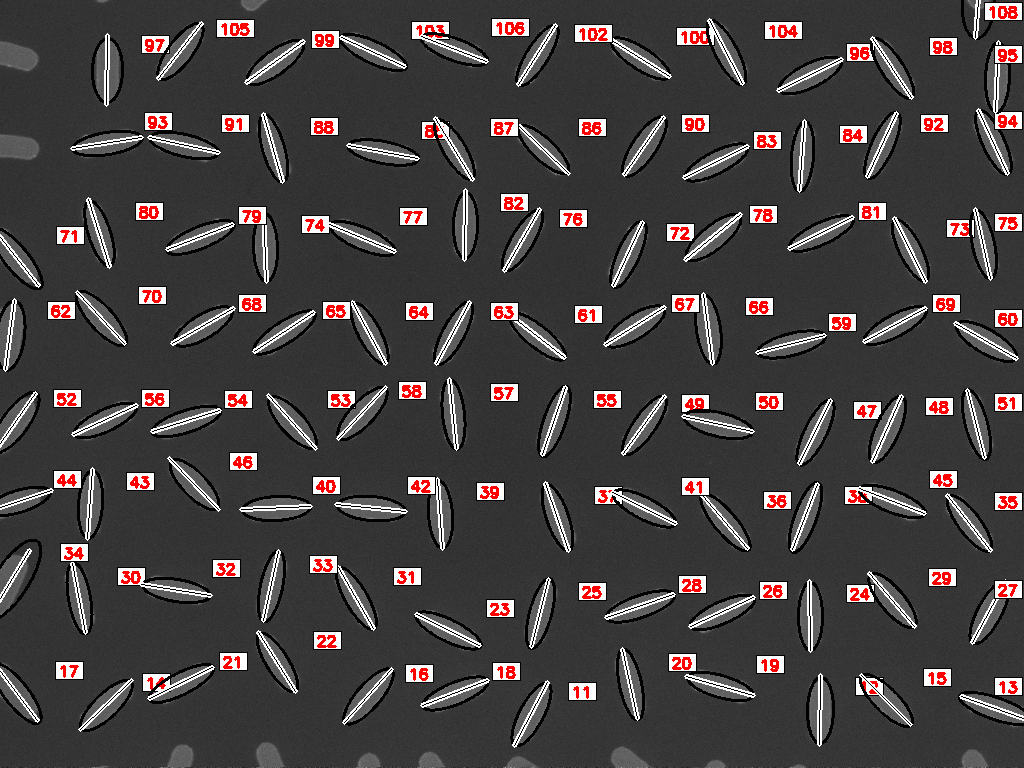
\includegraphics[width=\linewidth]{fig/overlay_with_ellipses.png}
        \caption{}
        \label{fig:sac1b}
    \end{subfigure}

    \caption{The arrangement of nanoparticles in Fig.1 in \cite{Saccone2022}. (a) Original picture, (b) Image processing for particle position and orientation of their easy axes. Recovered shape of particles is shown by black elliptical outline for each particle. The long axis of an ellipse indicates the easy axis of the particle. Every particle is numbered by its center position from bottom to top for further filtering and consisting sub-lattices. Some truncated particles are filtered with an appropriate condition.}
    \label{fig:sac1}
\end{figure*}

We analyzed the image for arrangement of particles Fig.1 in \cite{Saccone2022} (Fig.~\ref{fig:sac1a}) and found that the distance between nearest particles is $r = 326 \pm 33$ nm. 

We perform an image processing to get size of nanoparticles and orientation of their easy axes. 
cv2 python library has been used. The shape of particle is supposed as ellipse, though it is more similar to bacillus or rod shape. Figure~\ref{fig:sac1b} shows the result of the image processing. 

We can see some particles truncated by the frame of image. Those particles should be filtered, for example, by setting the limit size of ellipse: with lower limit of long axis 60 pixel, we select 95 ellipses among 109 ``recognized'' ellipses in Fig.~\ref{fig:sac1b}. Considering that the mean long axis is 71 pixels and the real size is claimed to be 300 nm, the lower limit seems to be 250 nm. The orientation of easy axes could be supposed to be uniformly distributed, whence the system seems isotropic. 

Now, let's inspect the tendency of the physical properties like the heat capacity and magnetic susceptibility along with the increase of the size of the lattice. Then we can infer if those quantities diverge in the system of the thermodynamic limit. Hereafter, particles and spins are treated as having the same meaning.

If we are going to inspect the system of the size of 3, we can select 9 nearest or contagious particles to compose $3\times3$ sub-lattice, for example: $97\ 105\ 99\ |\ 93\ 91\ 88\ |\ 80\ 79\ 74$ in Fig.~\ref{fig:sac1b}, where the numbers indicate the particles. In the above configuration, we can compose 54 instances of such $3\times3$ sub-lattices, 41 $4\times4$ sub-lattices, 26 $5\times5$ sub-lattices, 16 $6\times6$ sub-lattices, 9 $7\times7$ sub-lattices, 4 $8\times8$ sub-lattices.

As mentioned above, in the system the flip of spin is allowed. Taking into account all possible flips, for example, for a $3\times3$ sub-lattice, there are $2^{3\times3}$ = 512 states like $\{-1, 1, -1; 1, 1, -1; -1, 1, -1\}$ and for a $4\times4$ sub-lattice, there are $2^{4\times4} = 65536$ states like $\{1, 1, -1, 1; -1, 1, 1, 1; 1, 1, -1, -1\}$. The sign of the spin depends on the initial state. In the enumeration method, all $2^{N\times N}$ (where $N$ is the number of spins) flipped spin states are considered. Once a temperature is given, each state has a weight given $\exp(-\beta E)$, where $\beta = 1/k_BT$ and $E$ is the energy of the state. This weight means a probability of realization of the state. Therefore, we can estimate a physical quantity such as the energy or the total spin by thermal averaging, that is, with the weight $\exp(-\beta E)$. 

In Monte-Carlo (MC) method, a Metropolis approach is applied. We give a state randomly, then choosing spins randomly and flipping them. Calculate the energy of the previous state (before flip) and the new state (after flip). If the energy of the new state is lower, then the new state is accepted and inserted to the process of `realized' states. If the energy of the new state is greater, then the new state is accepted or inserted to the process with the rate of $\exp(-\beta E)$. This approach provides scanning `all' states and the realization factor $\exp(-\beta E)$ for each state within the process. In other words, inspecting the process, we can find a state with the frequency scaling as $\exp(-\beta E)$. Therefore, simply averaging over the states in the process, we could get a `thermal average' of the quantities as in the enumeration.

It is possible to perform simulation by enumeration and MC for $3\times3$, $4\times4$ and $5\times5$ sub-lattices. For size of 6 to 8, Monte-Carlo simulation is performed. We conclude the resultant properties by averaging the instances for each size of sub-lattice. 


% ============================================================
\section{Results}
\label{sec:results}
Here we consider the heat capacity and the magnetic susceptibility per spin because those quantities are volume-dependent. 

Figure~\ref{fig:capSac} shows the temperature vs. the heat capacity averaged over the instances of sub-lattice of various sizes calculated in the enumeration and MC methods, respectively. The curves are very close. 

\begin{figure*}[t]
    \centering
    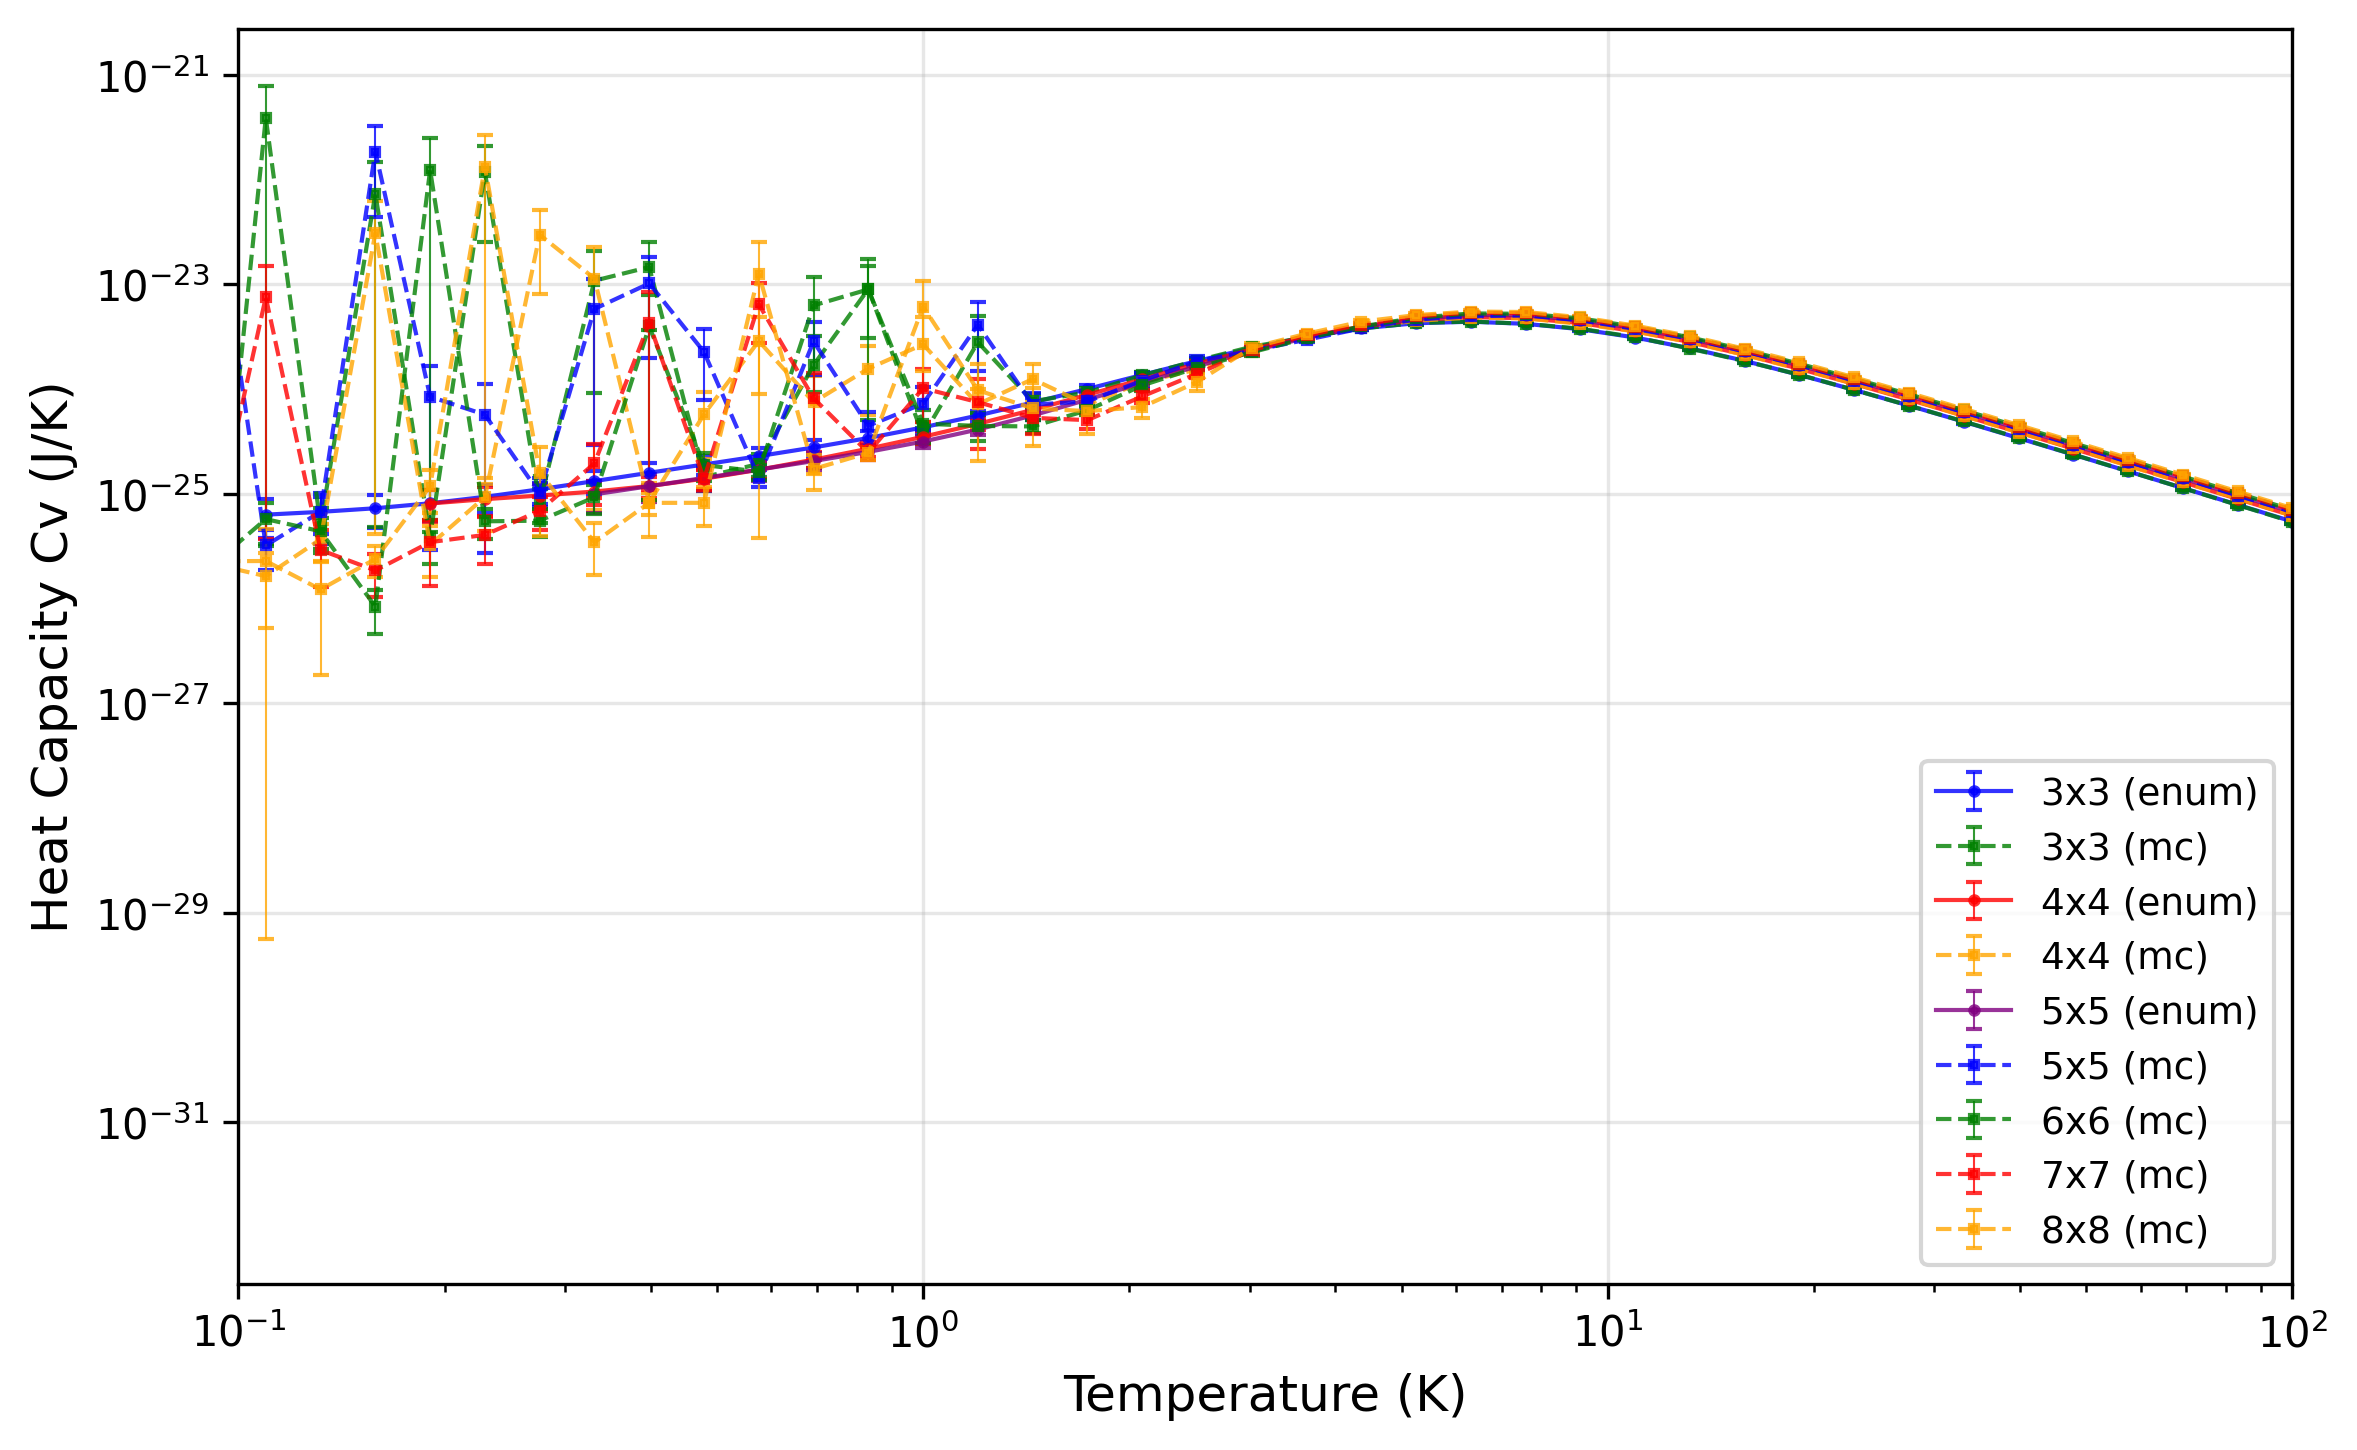
\includegraphics[width=1.5\columnwidth]{fig/heat_capacity_comparison.png}
    \caption{Temperature vs heat capacity in sub-lattices of various sizes calculated by the enumeration and Monte-Carlo method.  Peaks in lower temperature appear in only Monte-Carlo method so could be ignored. A small shift is found between curves.}
    \label{fig:capSac}
\end{figure*}

On the other hand, Fig.~\ref{fig:invSusSac} shows a Curie-Weiss (CW) behavior appears in magnetic susceptibility of the considered sub-lattices. The asymptotes are observed in the inverse susceptibility. We consider both types of susceptibilities: for the total spin of system and for its y-component (tau). They all show CW behavior with a bit different CW temperature.  

\begin{figure*}[t]
    \centering

    % ---- Subfigure (a) ----
    \begin{subfigure}[b]{0.4\textwidth}
    	%\adjincludegraphics[width=\linewidth]{fig/Inverse_chi_spin.png}
        % \includegraphics[width=\linewidth]{fig/Inverse_χ_spin.png}
        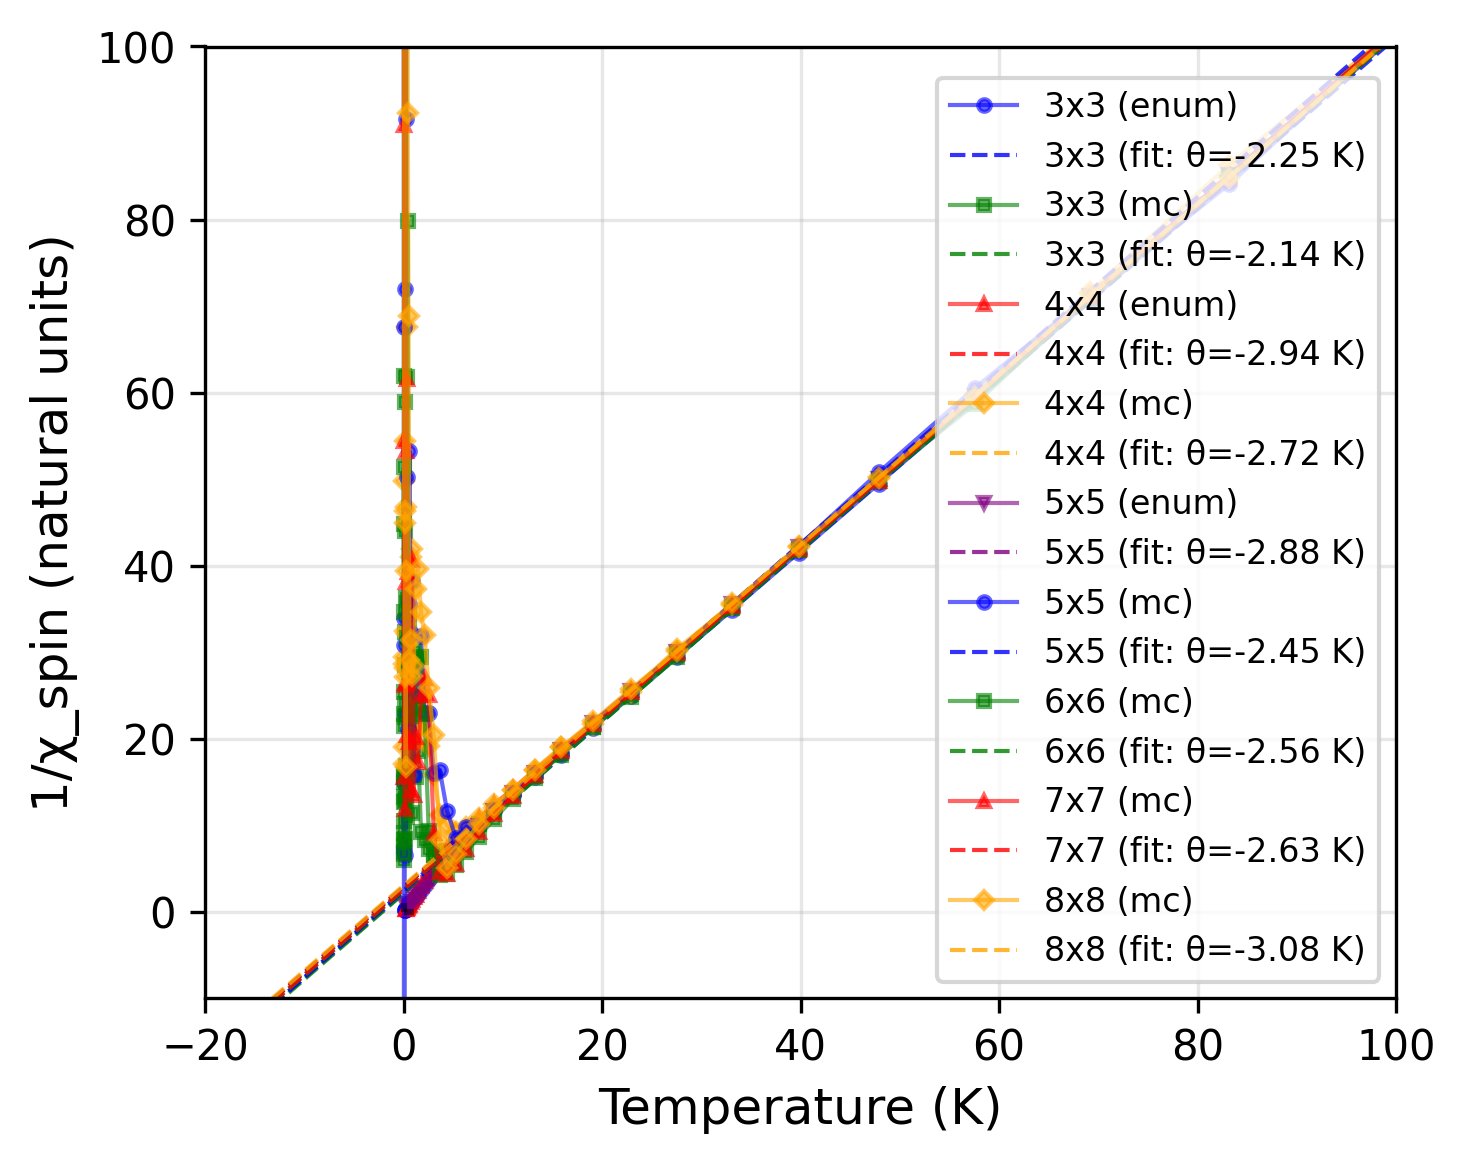
\includegraphics[width=\linewidth]{fig/Inverse_chi_spin.png}
        \caption{}
        \label{fig:invSusSaca}
    \end{subfigure}
    \quad
    % \hfill
    % ---- Subfigure (b) ----
    \begin{subfigure}[b]{0.4\textwidth}
        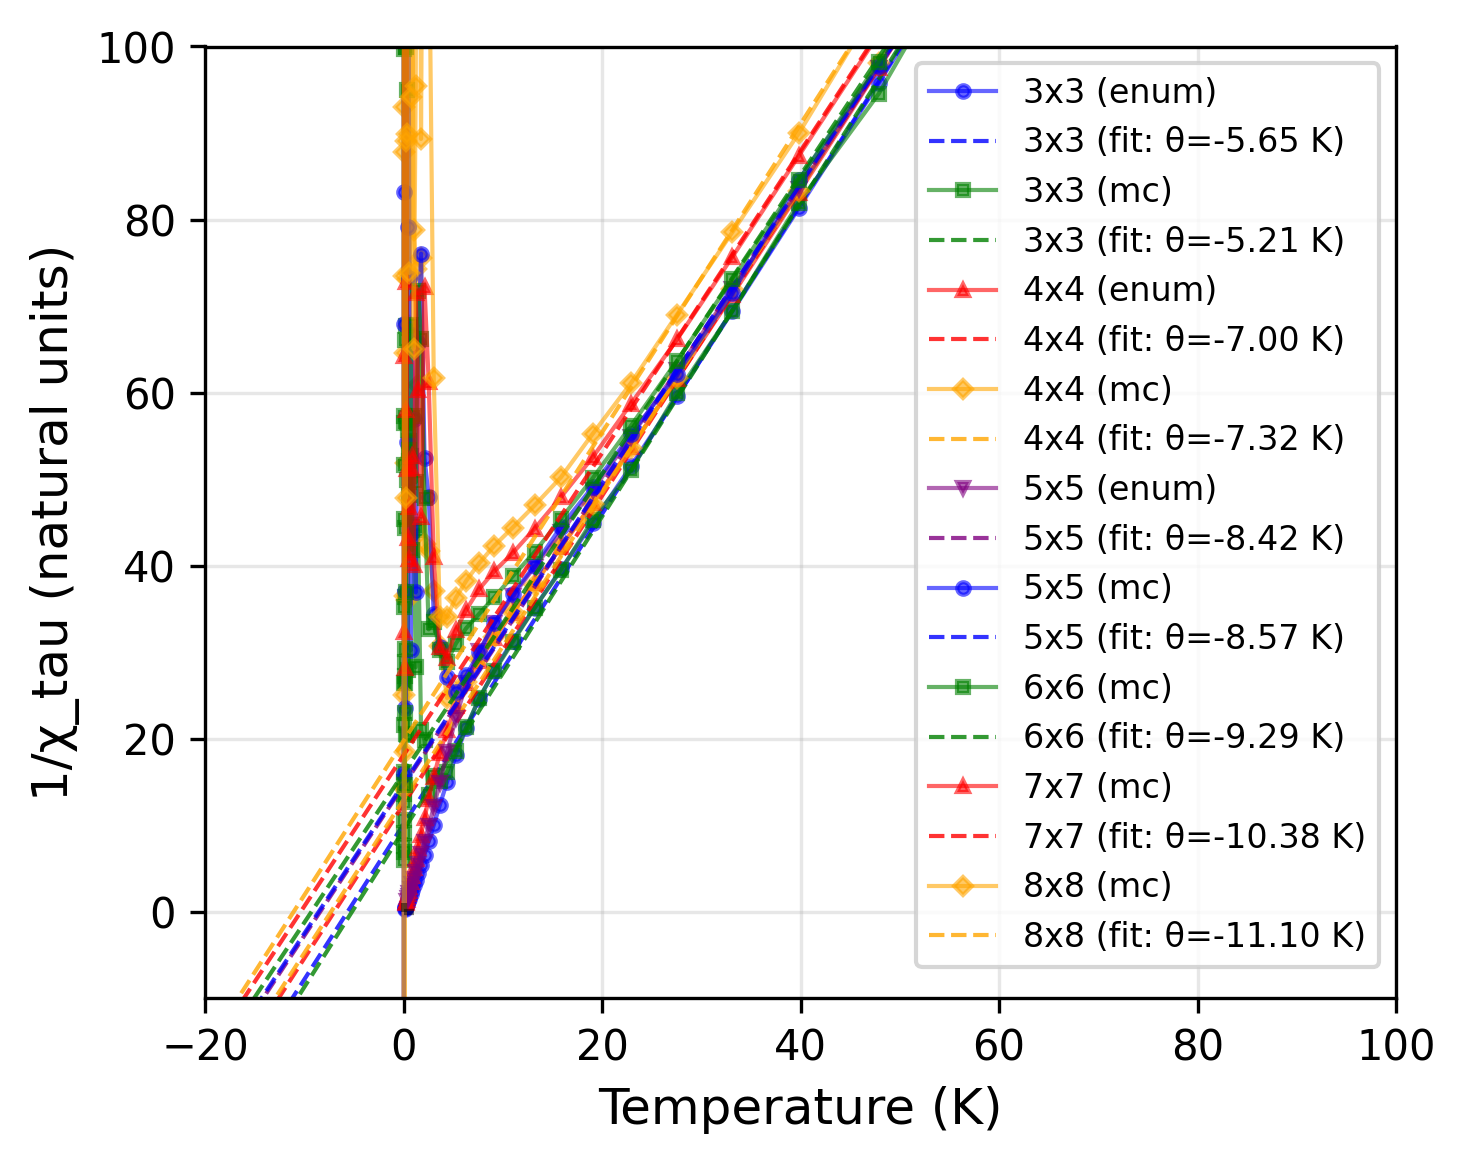
\includegraphics[width=\linewidth]{fig/Inverse_chi_tau.png}
        \caption{}
        \label{fig:invSusSacb}
    \end{subfigure}

    \caption{The temperature vs. the inverse susceptibilities and their Curie-Weiss behavior. (a) The inverse susceptibility for the total spin. (b) The inverse susceptibility for the total y-component. The legends shows the size of sub-lattice, applied method and Curie-Weiss temperature. The natural units can be found in Appendix~\ref{app:natUnit}.}
    \label{fig:invSusSac}
\end{figure*}

In summary, we could study how the peak height of the heat capacity and the susceptibility change with the size of sub-lattice or if the peak diverges in the thermodynamic lattice. Figure~\ref{fig:maxSac} shows how the maxima change with the size of sub-lattce. In Fig.~\ref{fig:maxSaca} we can expect that the peak of the heat capacity raises with the size, which means that the peak could diverge in the thermodynamic limit. For the susceptibilities such a divergence is not expected or even the peak of the tau (y-component) susceptibility could lower(?). Recall that the total heat capacity and susceptibility scale as the number of spins so that we evaluate the quantities per spin to discover the genuine divergence of the maxima. 

\begin{figure*}[t]
    \centering

    % ---- Subfigure (a) ----
    \begin{subfigure}[b]{0.3\textwidth}
        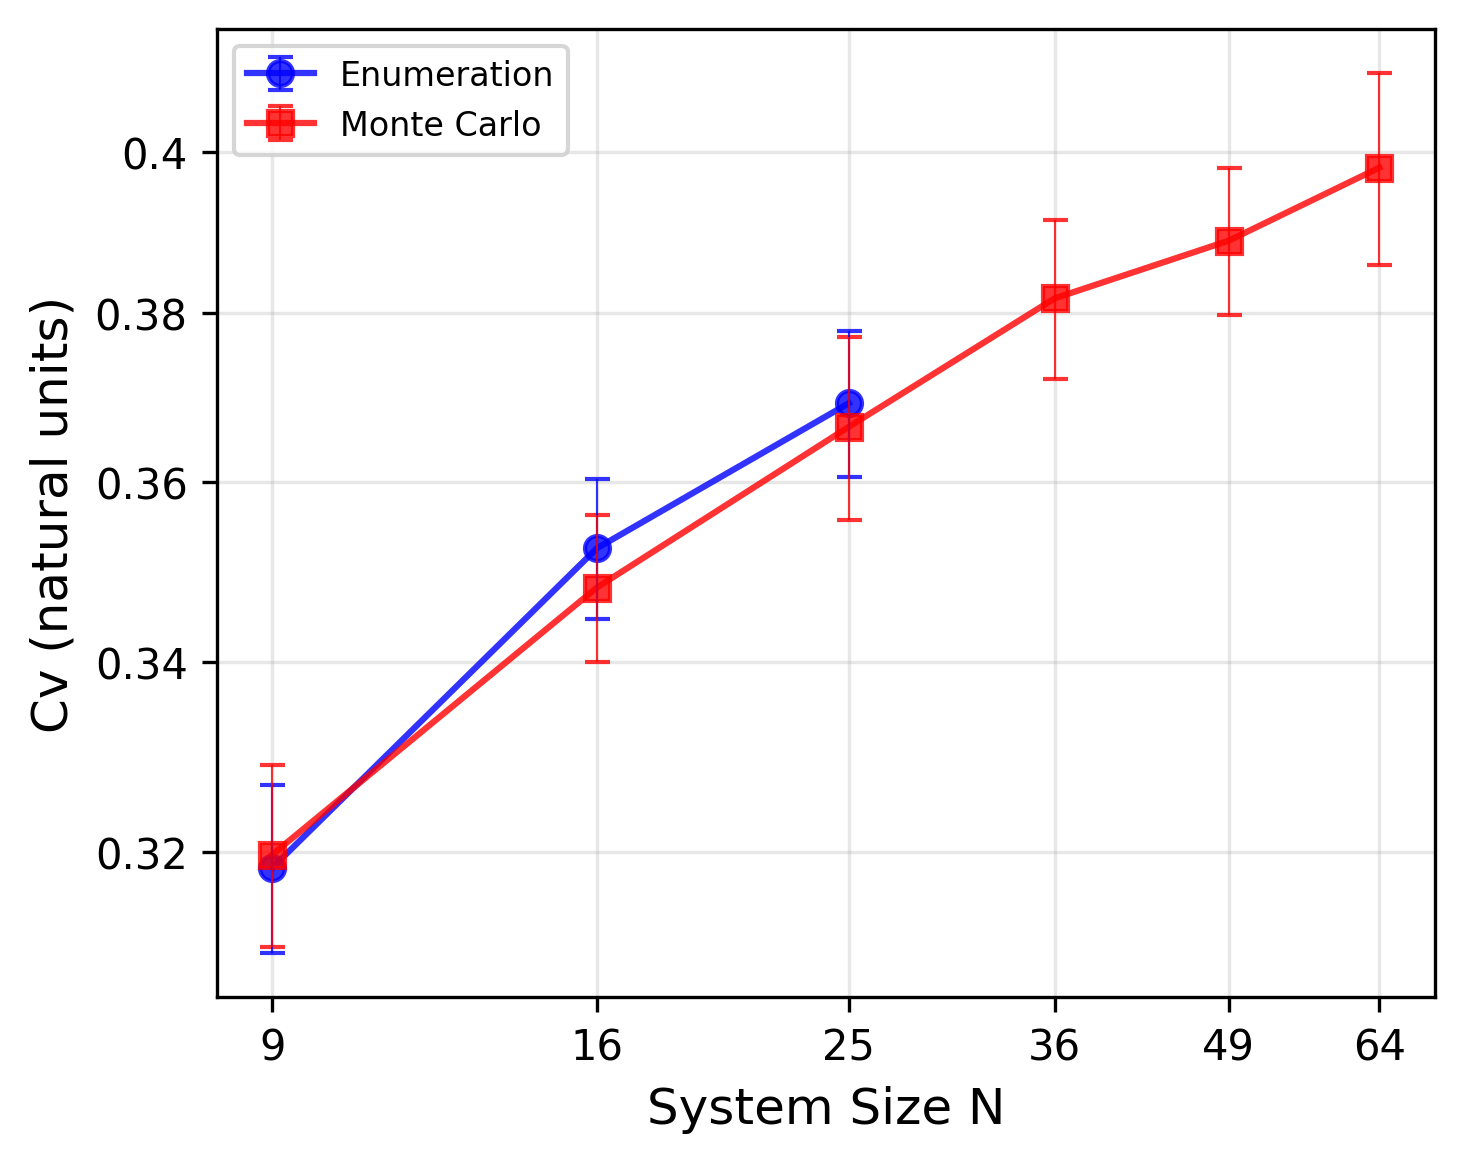
\includegraphics[width=\linewidth]{fig/Heat Capacity Peak.png}
        \caption{}
        \label{fig:maxSaca}
    \end{subfigure}
    \quad
    % \hfill
    % ---- Subfigure (b) ----
    \begin{subfigure}[b]{0.3\textwidth}
        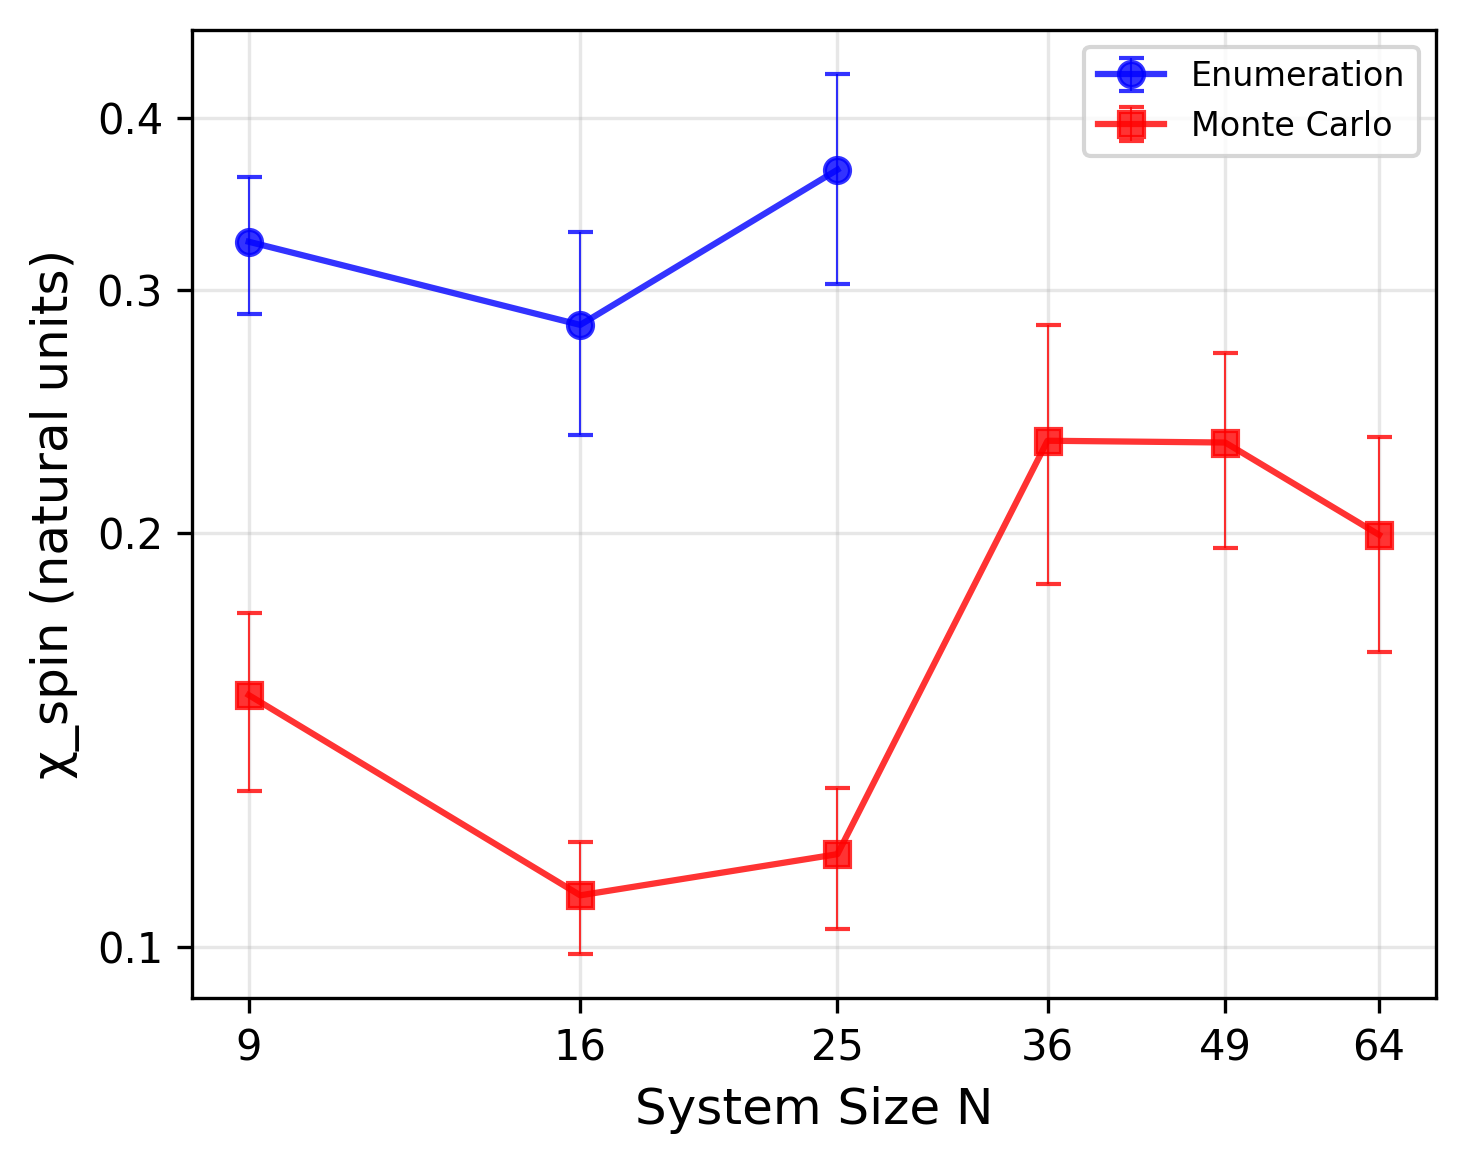
\includegraphics[width=\linewidth]{fig/Spin Susceptibility Peak.png}
        \caption{}
        \label{fig:maxSacb}
    \end{subfigure}
    \quad
    % \hfill
    % ---- Subfigure (c) ----
    \begin{subfigure}[b]{0.3\textwidth}
        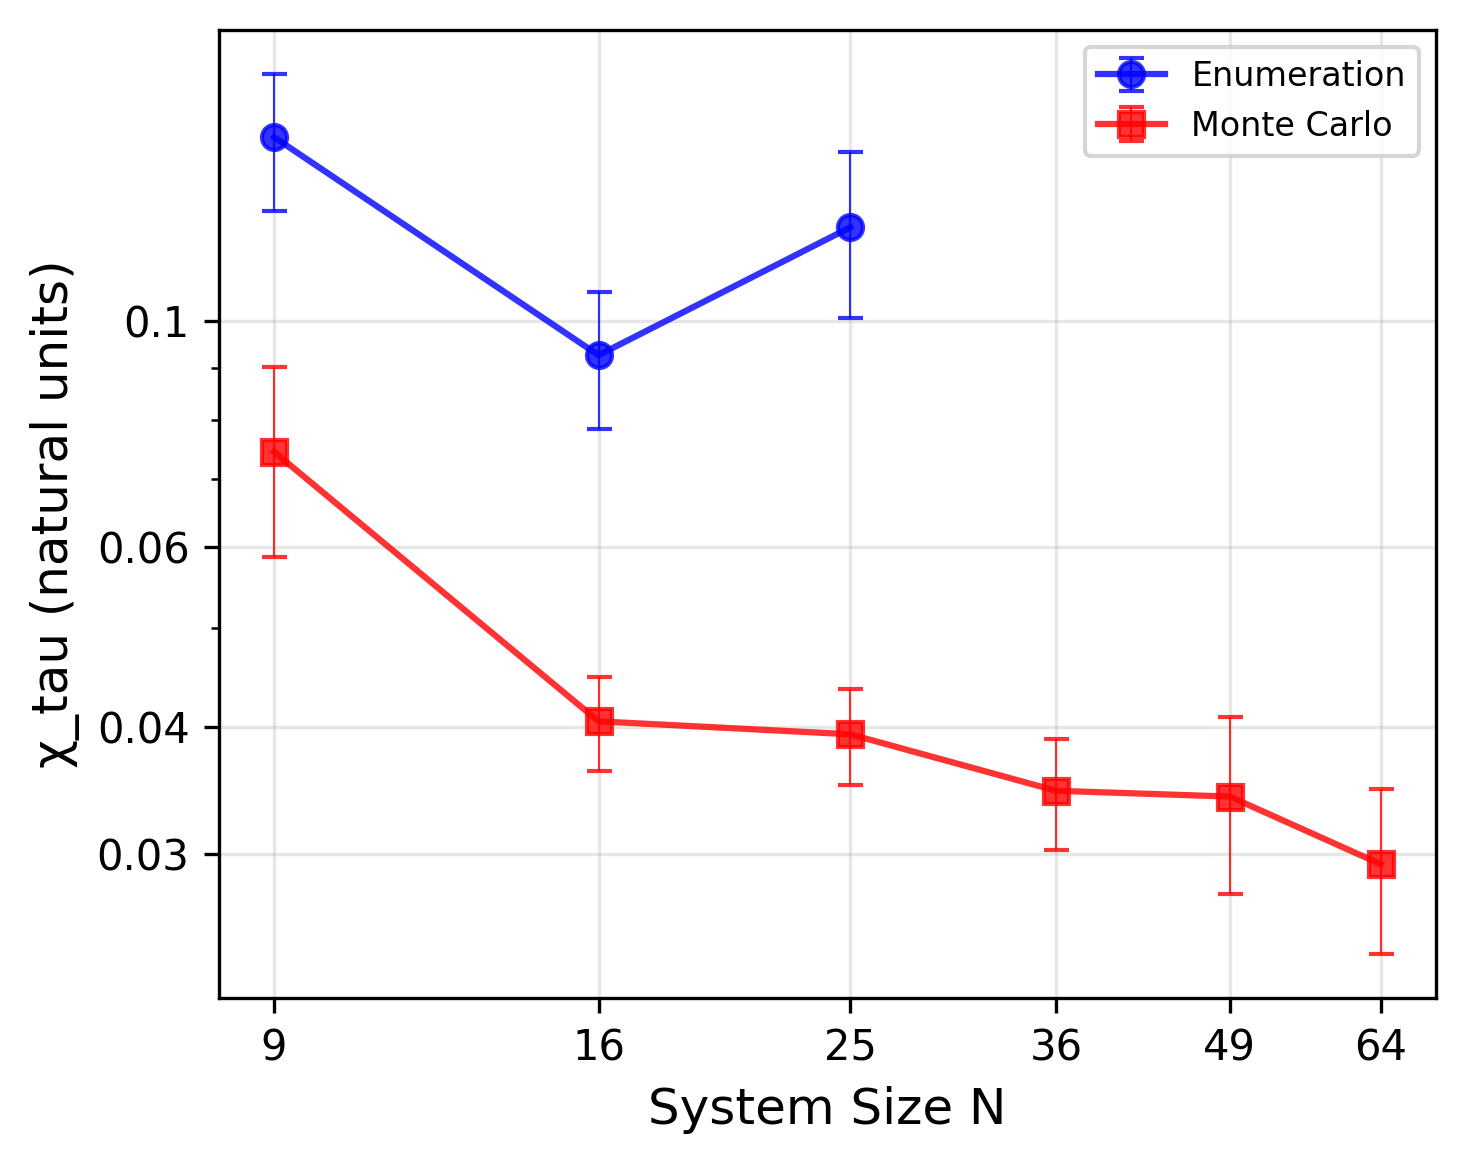
\includegraphics[width=\linewidth]{fig/Tau Susceptibility Peak.png}
        \caption{}
        \label{fig:maxSacc}
    \end{subfigure}
    
    \caption{The change of maxima of the heat capacity and the susceptibilities per spin with the size of sub-lattice. (a) The change of peak height of the heat capacity. (b) The change of peak height of the susceptibility for the whole spin. (c) The change of peak height of the susceptibility for the y-component spin. The error bar corresponds to the statistics over all the sub-lattices of the same size. The natural units can be found in Appendix~\ref{app:natUnit}.}
    \label{fig:maxSac}
\end{figure*}

We consider such a divergence in relation to the degeneration of the ground state. If the degree of degeneration of the ground state is 1 or 2, in other words, if the degree is too small, crossover (or phase transition ?) is expected. In fact, the Density of States (DOS) diagram (Fig.~\ref{fig:DOSSac}) shows that the degree of degeneration of the ground state in size of 3 and 4 is 2 and 1, which means that a crossover could occur in those cases. In the crossover, the physical quantities do not diverge or keep constant while in the phase transition, the quantities diverge. 

\begin{figure*}[t]
    \centering

    % ---- Subfigure (a) ----
    \begin{subfigure}[b]{0.4\textwidth}
        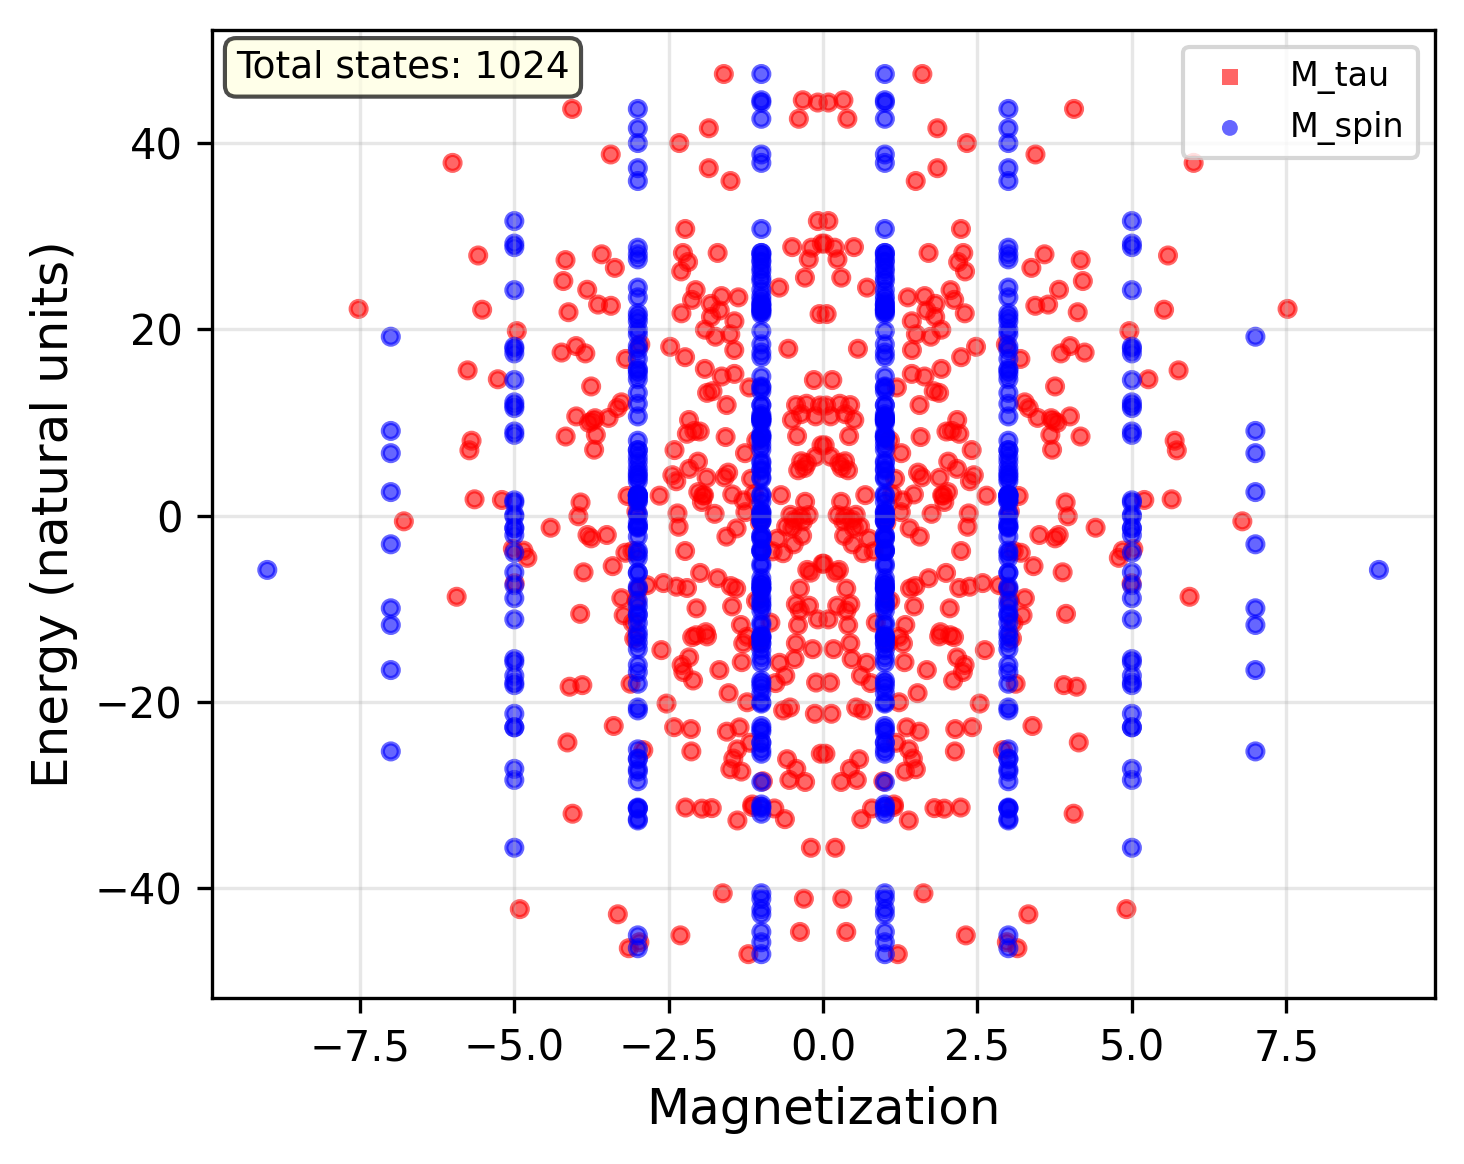
\includegraphics[width=\linewidth]{fig/MEG 3.png}
        \caption{}
        \label{fig:DOSSaca}
    \end{subfigure}
    \quad
    % \hfill
    % ---- Subfigure (b) ----
    \begin{subfigure}[b]{0.4\textwidth}
        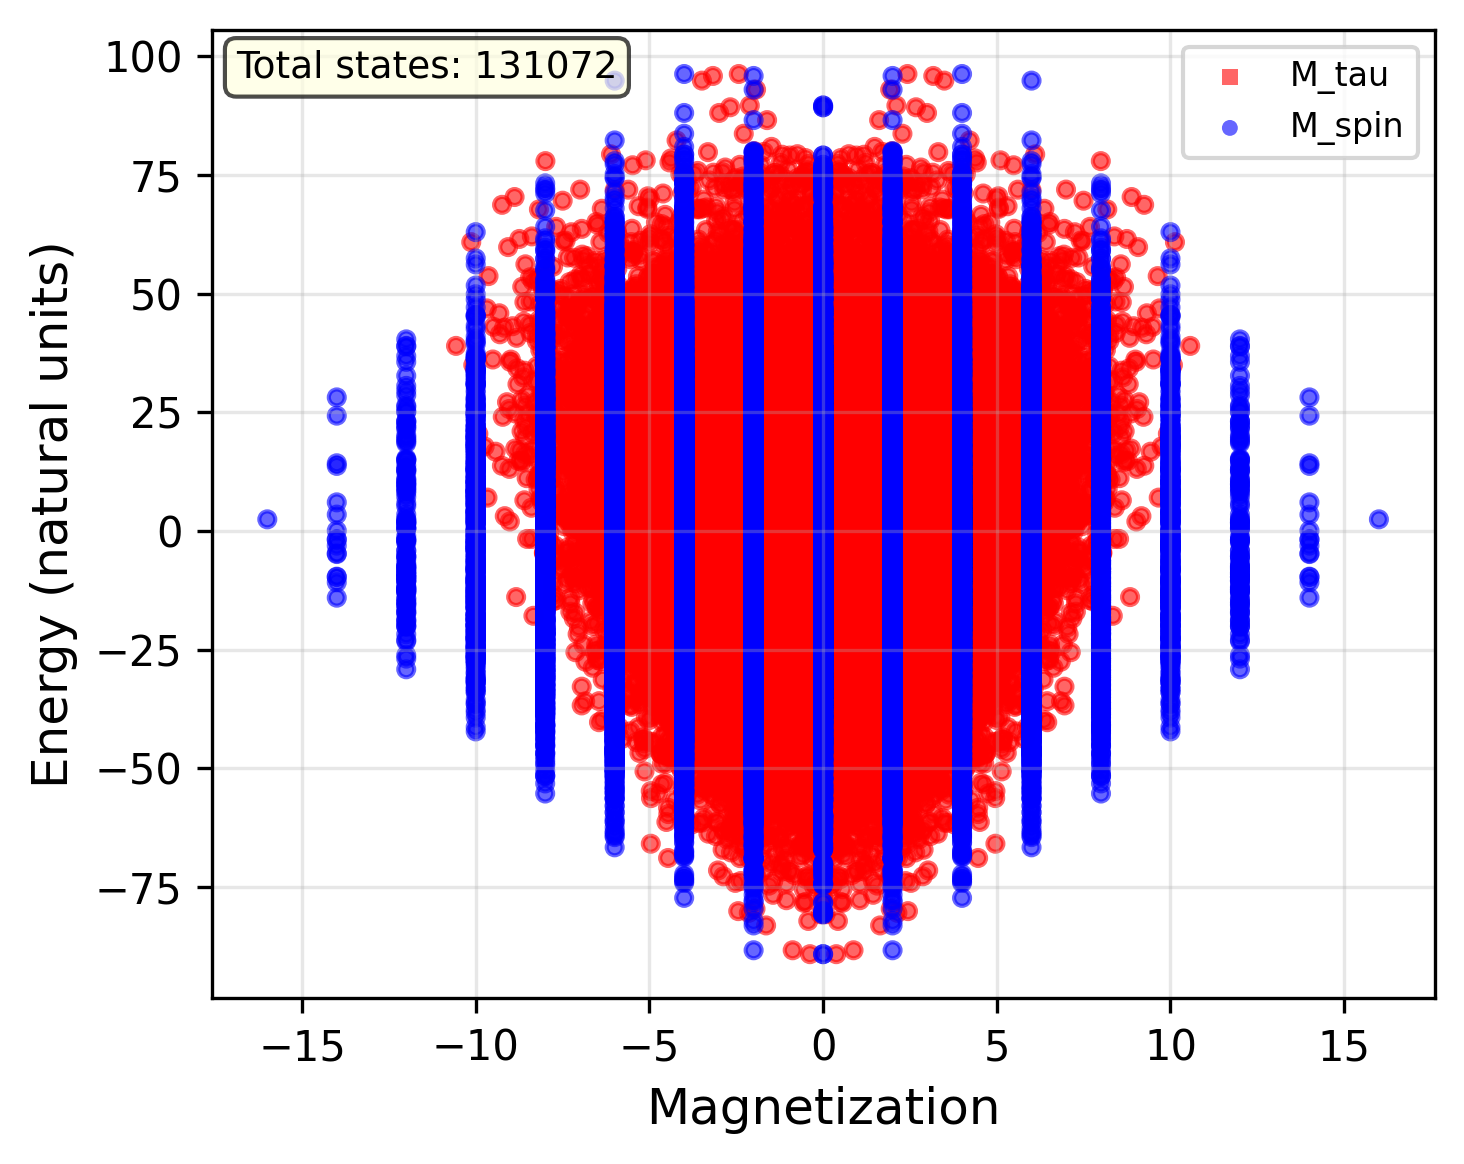
\includegraphics[width=\linewidth]{fig/MEG 4.png}
        \caption{}
        \label{fig:DOSSacb}
    \end{subfigure}
    
    \caption{Energy vs. magnetization in DOS diagrams for sub-lattices of size 3 and 4. (a) The size of 3, (b) The size of 4. Red points stand for the magnetization for a state composed of the whole spins and blue points for the magnetization of the tau spins. The ground state (of the lowest energy) is 2-fold degenerated in the size of 3 and not degenerated in the size of 4. The natural units can be found in Appendix~\ref{app:natUnit}.}
    \label{fig:DOSSac}
\end{figure*}



% ============================================================
\section{Conclusions}
\label{sec:conclusions}



% ============================================================
\begin{acknowledgments}
We thank ... for helpful discussions. This work was supported by ...
\end{acknowledgments}

% ============================================================
\appendix

\section{Natural units}
\label{app:natUnit}

We set $k_B=1$ and consist the natural units for the quantities (Table A1.1), considering the following constants, where $T_0 = 1$K is a conventional constant and other units, especially the temperature, depend on it:

$\mu_0 = 4\pi \times 10^{-7}$ H/m,

$k_B = 1.38 \times 10^{-23}$ J/K,

$\mu_{ref} = 5.41 \times 10^{-18}$ Am$^2$,

$J_{0}=k_{B}T_{0}$ [J], 

$a={\left(\frac{{\mu }_{0}\text{\,}{\mu }_{\text{ref}}^{2}}{4\pi \text{\,}k_{B}\cdot T_{0}}\right)}^{1/3}=5.9626\times {10}^{-7}\text{\ m}=5.9626\text{\ nm}$.

\begin{table*}[t]
    \centering
    \caption{The SI and natural units of the main quantities}
    \label{tab:natUnits}
    \begin{ruledtabular}
    \begin{tabular}{lccc}
        Quantity $q$ & SI units & Natural units & $q_{\text{SI}}$/$q_{\text{natural}}$\\
        \hline
        Temperature $T$	& K & -$^a$ & 1 [K] \\
        Energy $E$	& J	& -$\;\;$	& $J_0$ \\
        Heat capacity per spin $Cv$	& J/K & -$\;\;$ & $k_B$ \\
        % Heat capacity per volume $Cv$ & J/(K$\cdot$m$^3$) & -$\;\;$ & $k_B/a^3$ \\
        Magnetic susceptibility per spin $\chi$ & m$^3$ & - & $4\pi a^3= \mu_0 \mu_{ref}^2/J_0$ \\
        % Magnetic susceptibility per volume $\chi$ & - & -$\;\;$ & 4$\pi$ \\
        Length (e.g. of correlation) $L$ & m & -$\;\;$ & $a$
    \end{tabular}
    \end{ruledtabular}
    \raggedright $^a$ - Dimensionless.
\end{table*}

% ============================================================
% Bibliography
% Two options:
%   (A) Inline \begin{thebibliography}{99} ... \end{thebibliography}
%   (B) BibTeX with \bibliography{refs}
% ============================================================

% ---------- Option A: inline bibliography ----------
\begin{thebibliography}{99}

\bibitem{Saccone2022}
Michael Saccone, Francesco Caravelli, Kevin Hofhuis, Sergii Parchenko, Yorick A. Birkhölzer, Scott Dhuey, Armin Kleibert, Sebastiaan van Dijken, Cristiano Nisoli \& Alan Farhan, Direct observation of a dynamical glass transition in a nanomagnetic artificial Hopfield network. Nat. Phys. \textbf{18}, 517–521 (2022). https://doi.org/10.1038/s41567-022-01538-7

 \bibitem{EA1975} Sir Sam Edwards and Philip W. AndersonTitle, Theory of spin glasses, Journal of Physics F: Metal PhysicsYear: 1975, 5, 5, 965–974, DOI: 10.1088/0305-4608/5/5/017

\end{thebibliography}

% ---------- Option B: BibTeX (uncomment) ----------
% \bibliography{refs}

\end{document}
